\documentclass[english]{exercisesheet}

\usepackage{bm}
\usepackage{mymath}
\usepackage{graphicx}

\author{Lorenzo Minecci, Daniel Strenger}
\immatriculationnumber{11939539, 01531211}
\semester{SS 2020}
\subject{Machine Learning}
\sheetnumber{2}

 \begin{document}
 \makedocumentheader
  \begin{nexercise}{Online Bayesian Linear Regression}
  \begin{solution} 1.
  
  \begin{align*}
  p(t|\bm{x}, \bm{w}) = \prod_{n=1}^N \sqrt{\frac{\beta}{2\pi}}\exp{(-\beta \frac{( \bm{t}-\bm{w}^{T} \bm{\phi}(x_n))^{2}}{2})}
  \end{align*}
  \begin{align*}
      \log(p(\bm{t}|\bm{x}, \bm{w})) = \sum_{n=1}^N \frac{1}{2}(\ln{\beta}-\ln{2\pi}) + [-\frac{\beta}{2}(\bm{t}-\bm{w}^{T}\bm{\phi}(x_{n}))^{2}] = \frac{N}{2}(\ln\beta-\ln2\pi)-\beta\underbrace{\frac{1}{2}\sum_{n=1}^N(\bm{t}-\bm{w}^{T}\bm{\phi}(x_{n}))^{2}}_\text{Ed}= 
  \end{align*}
  \begin{align*} \frac{N}{2}(\ln\beta-\ln2\pi)-\beta E_{D}
  \end{align*}
  \end{solution}
  
  \par 
  \begin{solution} 2.
  \\ It's a multivariate Gaussian, and again we are going to compute the logarithm. So:
  \begin{align*}
  \ln(p(\bm{w})) = \ln(\mathcal{N}(\bm {w} | \bm {0}, \alpha^{-1}I)) =  \frac{1}{(2\pi)^{\frac{D}{2}}\alpha^{-1}I}\exp\left((-\frac{1}{2}\bm{w}^{T}(\alpha^{-1}I)\bm{w})\right) = \\ -\frac{D}{2}\ln(2\pi)-\frac{1}{2}\ln(|\alpha^{-1}I|)-\left(\frac{1}{2}\bm{w}^{T}(\alpha^{-1}I)^{-1}\bm{w}\right) = 
  \end{align*}
  In this setting we notice that only the third term is dependent on $w$, while the first two terms as constants. We'll use this consideration for the next exercise.
    \end{solution}\\
    \begin{solution} 3.
  \par 
  Bayes theorem states that:
  \begin{align*}
  p(\bm{w}|\bm{t}) = \frac{p(\bm{t}|\bm{w})p(\bm{w})}{p(\bm{t})}
  \end{align*}
  We assume that $p(\bm t)$ is not depending on $w$, so also its logarithm will be independent. \\ Let's compute the logarithm of the posterior simply as:
  \begin{align*}
      \ln(p(\bm{t}|\bm{w}))+ \ln(p(\bm{w})) + cost = \underbrace{\frac{N}{2}\left(\ln\beta-\ln(2\pi)\right)}_\text{cost} - \frac{\beta}{2}\sum_{n=1}^{N}(\bm{t}-\bm{w}^{T}\bm{\phi}(x_{n}))^{2} + \\ + \left[\underbrace{-\frac{D}{2}\ln(2\pi)-\frac{D}{2}\ln(\alpha)}_\text{cost}+\left(-\frac{1}{2}\bm{w}^{T}(\alpha^{-1}I)^{-1}\bm{w}\right)\right] = \\
      \end{align*}
      concluding:
     \begin{align*}
      \ln(p(\bm{w}|\bm{t})) = -\frac{\beta}{2}\sum_{n=1}^{N}(\bm{t}-\bm{w}^{T}\bm{\phi}(x_{n}))^{2}-\frac{\alpha}{2}\bm{w}^{T}\bm{w} + cost
    \end{align*}
    where we grouped in $cost$ all the terms constant with respect to $w$. The alpha becomes a scalar multiplying the vector product.
    The maximization of this distribution w.r.t. $\bm{w}$ is equivalent to the minimization of the sum-of-squares approach with addition of a quadratic regularization term $\lambda = \frac{\alpha}{\beta}$. \\
      \end{solution}
      \par
      \begin{solution} 4.\\
      Let's now maximise the log-posterior w.r.t. $w$
      We can express the vectors $\phi(x_{i})$ as rows of the design matrix $\Phi$
      \begin{align*}
          \frac{\partial}{\partial w_{i}}\left[\frac{\beta}{2}\sum_{n=1}^{N}(\bm{t}-\bm{w}^{T}\bm{\phi}(x_{n}))^{2}-\frac{\alpha}{2}\bm{w}^{T}\bm{w}+cost \right] = \frac{\beta}{2}(2\Phi_{i}^{T}\Phi \bm{w} - 2\Phi_{i}^{T}\bm{t}) + \frac{\alpha}{2}2\bm{w} = \\ = \left(\beta\Phi^{T}\Phi+\alpha I\right)\bm{w}-\beta\Phi_{i}^{T}\bm{t} \stackrel{!}{=} 0 \\
      \end{align*}
      \begin{align*}
          \Rightarrow \bm{w}_{map} = (\Phi^{T}\Phi + \frac{\alpha}{\beta}I)^{-1}\Phi \bm{t} \\
      \end{align*}
      That we can see it's equal to $\bm{m} = \beta\bm{S\Phi^{T}t}$, being $\bm{S}=\left(\alpha \bm{I} +\beta \bm{\Phi^{T}\Phi}\right)^{-1}$.\\ We took $\beta$ out of $\bm{S}$, which is finally a scalar multiplier in $\bm{m}$ .\\
      \end{solution}
 \end{nexercise}
 
 \begin{nexercise}{Logistic Regression}
\end{nexercise}

\begin{solution}
 1. We have $p(t=1|\bm{\tilde{x}})=\sigma(\bm{\tilde{w}}^t\bm{\tilde{x}})=\sigma(1\cdot\bm{w}^t\bm{\tilde{x}})$ and

 \begin{align*}
 p(t=-1|\bm{\tilde{x}})=1-\sigma(\bm{\tilde{w}}^t\bm{\tilde{x}})=1-\frac{1}{1+e^{-\bm{\tilde{w}}^t\bm{\tilde{x}}}}=\frac{1+e^{-\bm{\tilde{w}}^t\bm{\tilde{x}}}}{1+e^{-\bm{\tilde{w}}^t\bm{\tilde{x}}}}-\frac{1}{1+e^{-\bm{\tilde{w}}^t\bm{\tilde{x}}}}\\=\frac{e^{-\bm{\tilde{w}}^t\bm{\tilde{x}}}}{1+e^{-\bm{\tilde{w}}^t\bm{\tilde{x}}}}=\frac{1}{e^{\bm{\tilde{w}}^t\bm{\tilde{x}}}+1}=\sigma(-\bm{\tilde{w}}^t\bm{\tilde{x}})
\end{align*}\\
\par 2.
\begin{align*}
 -\log (p(\bm{\tilde{w}}|\bm{t},\bm{x}))=-\log(p(\bm{w}))-\sum_{n=1}^N \log(\sigma(t_n\bm{\tilde{w}^t\tilde{x}_n}))=\\-\log(p(\bm{w}))-\sum_{n=1}^N \log(\frac{1}{1+e^{-t_n\bm{\tilde{w}^t\tilde{x}_n}}})\\
 =-\log(p(\bm{w}))+\sum_{n=1}^N \log(1+e^{-t_n\bm{\tilde{w}^t\tilde{x}_n}})=\\-\log\left(\frac{1}{(2\pi S^{2})^{N/2}}\exp\left(-\frac{1}{2S^{2}}\sum_{n=1}^N w_n^2\right)\right)+\sum_{n=1}^N \log(1+e^{-t_n\bm{\tilde{w}^t\tilde{x}_n}})\\
 =-\log\left(\frac{1}{(2\pi S^{2})^{N/2}}\right)+\frac{1}{2S^{2}}\sum_{n=1}^N w_n^2+\sum_{n=1}^N \log(1+e^{-t_n\bm{\tilde{w}^t\tilde{x}_n}})
\end{align*}\\
\par 3.
\begin{align*}
 \frac{\partial}{\partial b}E(\bm{\tilde{w}})=\sum_{n=1}^N\frac{\partial}{\partial b} \log(1+e^{-t_n\bm{\tilde{w}^t\tilde{x}_n}})=\sum_{n=1}^N\frac{-t_ne^{-t_n\bm{\tilde{w}^t\tilde{x}_n}}}{1+e^{-t_n\bm{\tilde{w}^t\tilde{x}_n}}},\\
 \frac{\partial}{\partial w_i}E(\bm{\tilde{w}})=\frac{1}{2S^{2}}\sum_{n=1}^N  \frac{\partial}{\partial w_i} w_n^2+\sum_{n=1}^N\frac{\partial}{\partial w_i} \log(1+e^{-t_n\bm{\tilde{w}^t\tilde{x}_n}})\\
 =\frac{w_i}{S^{2}}+\sum_{n=1}^N\frac{-t_n\tilde{x}_n^ie^{-t_n\bm{\tilde{w}^t\tilde{x}_n}}}{1+e^{-t_n\bm{\tilde{w}^t\tilde{x}_n}}}
\end{align*}
\\
\par 5. b)
\begin{figure}[h]
\centering
 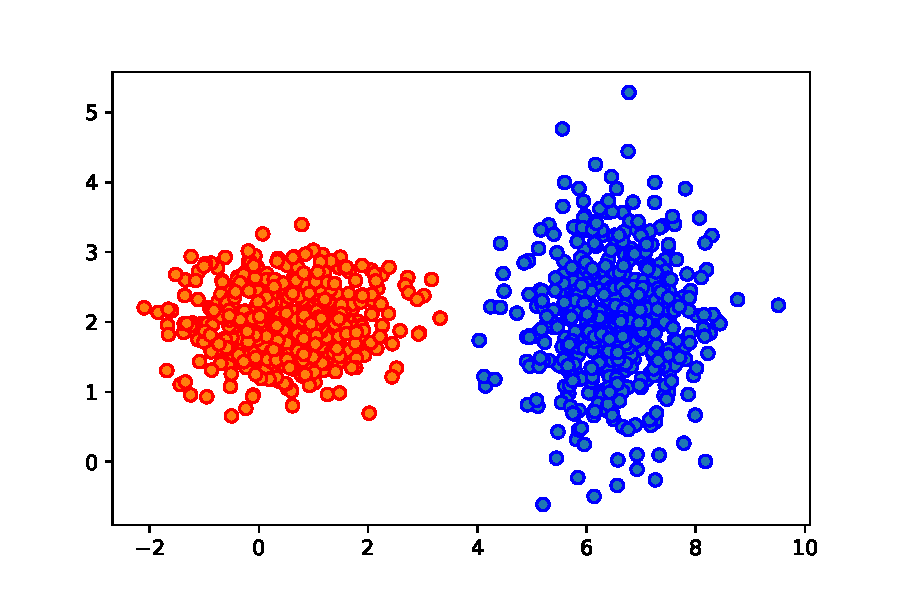
\includegraphics[width=0.7\textwidth]{points.pdf}
 \caption{The generated points}
\end{figure}

\par e,f) The decision boundary is the curve
\begin{align*}
 p(t=1|\bm{x})=0.5 \Leftrightarrow \frac{1}{1+e^{\bm{\tilde{w}^t\tilde{x}}}}=0.5\Leftrightarrow 1+e^{\bm{\tilde{w}^t\tilde{x}}}=2\Leftrightarrow \bm{\tilde{w}^t\tilde{x}}=\log(1)=0,
\end{align*}
so it is the line
\begin{equation*}
 y=-\frac{w_1}{w_2}x-\frac{b}{w_2}.
\end{equation*}

\begin{figure}
 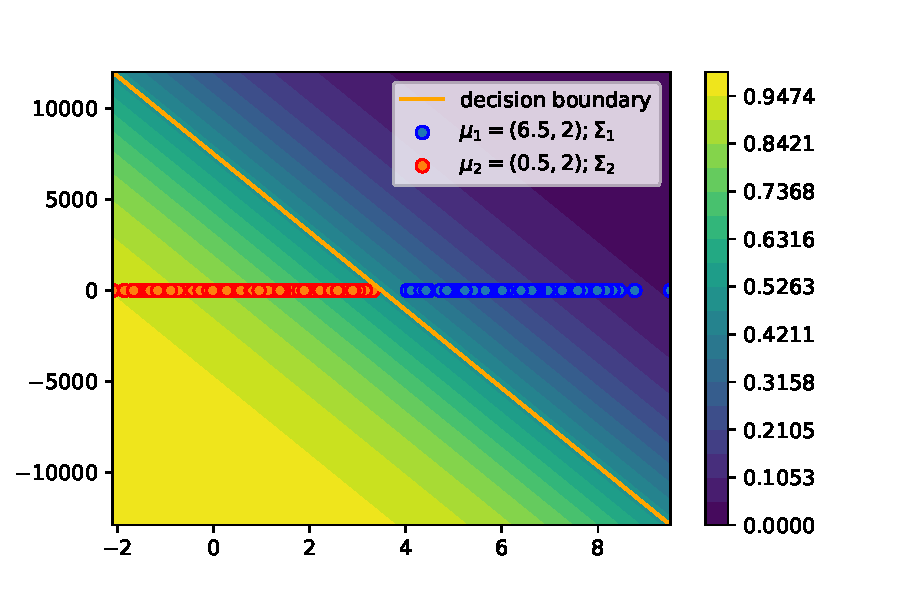
\includegraphics[width=0.5\textwidth]{simulated-1.pdf}
 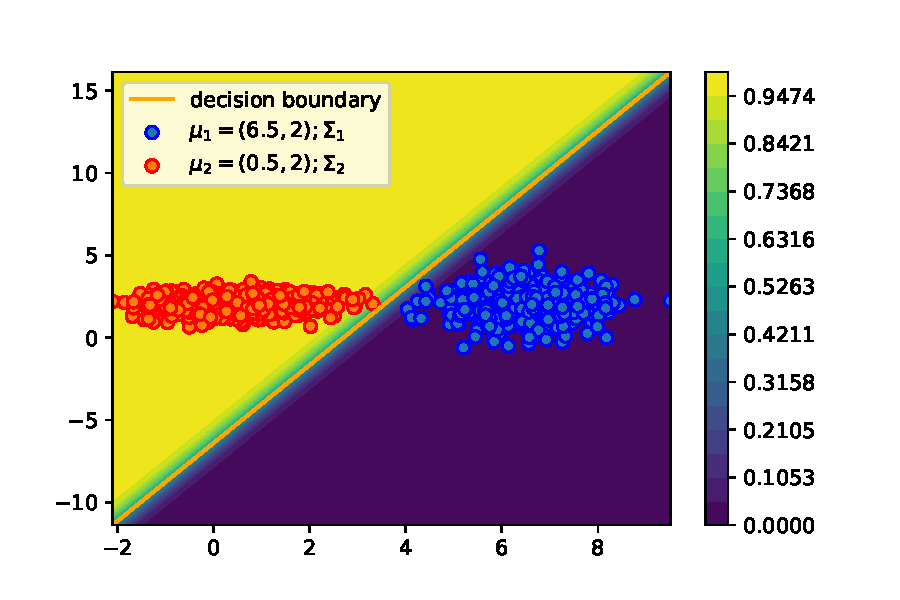
\includegraphics[width=0.5\textwidth]{simulated-8.pdf}
 \caption{decision boundary and probabilities for $S^2=10^{-3},10^4$}
\end{figure}
In this case the computed decision boundary really seperates the red and blue training points (for both values of $S^2$), although in some cases the points may not be linearly separable in two dimensions, which also happened in some tests. The probability around the decision boundary is about 0.5, which is clear, because the boundary was chosen for this reason. If a high variance for $\bm{w}$ is assumed, the probability decreases rather slowly when moving away from the decision boundary. For higher $S^2$ the probability decreases much faster and the predictions can be made with more certainty.\\
\par 6. The accuracy for variing $S^2$ is
\begin{table}[h]
\begin{tabular}{lll}
 $S^2$&training  &validation\\ \hline
 $10^{-4}$& 0.6088 & 0.6029 \\
 $10^{-3}$& 0.8435 & 0.8377 \\
 $10^{-2}$& 0.9003 & 0.8826 \\
 $10^{-1}$& 0.9193 & 0.9123 \\
 1& 0.9165 & 0.9152 \\
 $10^{1}$& 0.9169 & 0.9109 \\
 $10^{2}$& 0.9165 & 0.9145 \\
 $10^{3}$& 0.9143 & 0.9101 \\
 $10^{4}$& 0.9165 & 0.9138
\end{tabular}
\end{table}\\
It fits the previous observation that for higher $S^2$ the predictions can be made with more certainty, but this effect seems to be limited by $S^2 \approx 0.1$, after that no real improvement is achieved.
\end{solution}

 
\end{document}
